\documentclass{standalone}
\usepackage{Bachelor_Thesis_Institut_Neel/sty/themeKonstanz}
\begin{document}

    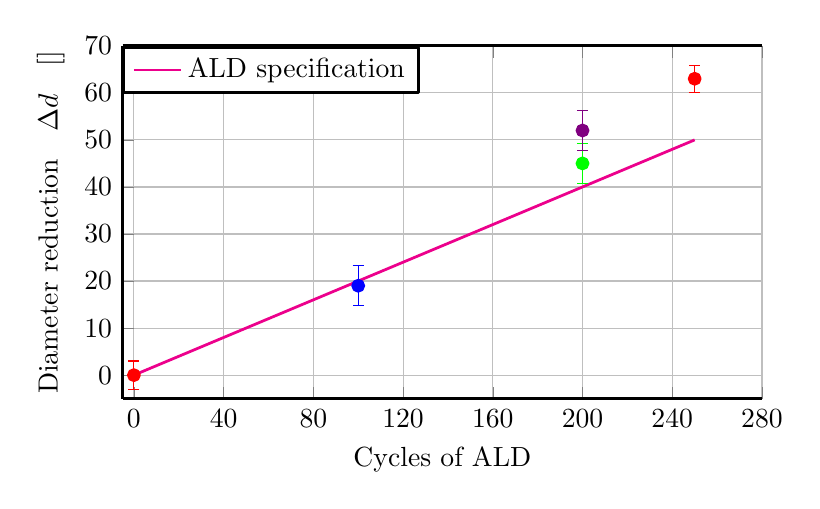
\begin{tikzpicture}
        \def\Xmin{-5}
        \def\Xmax{280}
        \def\Ymin{-5}
        \def\Ymax{70}
        \begin{axis}
            [
            /tikz/line join=bevel,
            width=0.8*\textwidth,
            height=0.5*\textwidth,
            axis y line*=left,
            line width = 1pt,
            xmin = \Xmin, xmax = \Xmax,
            ymin = \Ymin, ymax = \Ymax,
            xlabel = {Cycles of ALD},
            ylabel = {Diameter reduction$\quad \Delta d\quad[\si{\nano\meter}]$},
            xtick = {0,40,80,120,160,200,240,280},
            ytick = {0,10,20,30,40,50,60,70},
            grid,
            legend style={at={(0,1)}, legend columns=1, anchor=north west},
            ]
            %\addplot [color=blue, only marks,mark=o,]
            % plot [error bars/.cd, y dir = both, y explicit]
            % table[x=cycles, y=reduction, y error=error]{ALD_data.txt};
            \addplot[color=magenta, mark=none]
            coordinates {
            (0,0)
            (250,50)};
            \addlegendentry{ALD specification}
            \addplot [color=red, only marks, mark=*, mark options={solid},  error bars/.cd, y dir = both, y explicit]
            coordinates {
            (0, 0) +- (0,3)};
            \addplot [color=blue, only marks, mark=*, mark options={solid}, error bars/.cd, y dir = both, y explicit]
            coordinates {
            (100, 19) +- (0,4.24)};
            \addplot [color=green, only marks, mark=*, mark options={solid},  error bars/.cd, y dir = both, y explicit]
            coordinates {
            (200, 26+19) +- (0,4.24)};
            \addplot [color=violet, only marks, mark=*, mark options={solid}, error bars/.cd, y dir = both, y explicit]
            coordinates {
            (200, 52) +- (0,4.24)};
            \addplot [color=red, only marks, mark=*, mark options={solid},  error bars/.cd, y dir = both, y explicit]
            coordinates {
            (250, 63) +- (0,2.83)};
        \end{axis}

\end{tikzpicture}

\end{document}
